\section{La parallélisation du problème}

	Le problème \textit{stencil} que nous avions à traiter consiste à calculer la moyenne pondérée des quatre éléments adjacents pour chaque élément d'une matrice A. Le résultat est alors stocké dans une nouvelle matrice B. Dans notre programme, on effectue 200 fois cette itération.\\
	
	La parallélisation de la résolution problème doit faire intervenir le CPU mais aussi le GPU en les faisant coopérer. Pour ce faire la matrice doit être découpée en deux blocs. Un sera traité par le CPU et l'autre par le GPU. Une représentation schématique de cette division est présentée ci-dessous : 
	
	\begin{figure}[H]
		\centering
		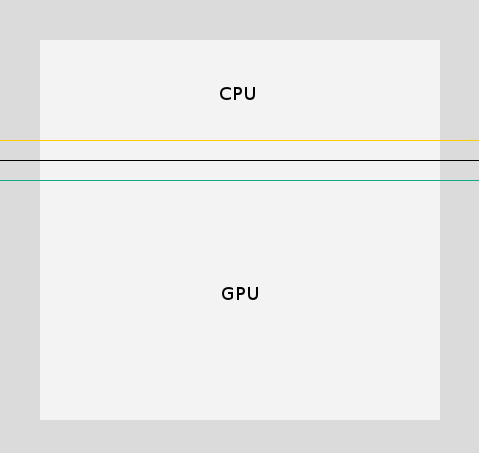
\includegraphics[scale=0.8]{schema.png}
		\caption{Schéma du partage de tâches entre CPU et GPU}
	\end{figure}
	
	
	La légende du schéma précédent est la suivante :
	
	\begin{itemize}
		\item Zone gris foncé : matrice originale avec bordures ajoutées artificiellement.
		\item Zone gris clair : matrice originale
		\item Trait noir : frontière de calcul CPU/GPU
		\item Trait jaune : délimiteur de la zone nécessaire au calcul sur GPU
		\item Trait vert  : délimiteur de la zone nécessaire au calcul sur CPU
	\end{itemize}
	
	Pour résoudre le problème du partage de la matrice entre les deux composants, nous avons fixé une limite appelée \verb?YDIM_GPU?. Cette limite correspond au nombre de lignes traitées par la carte graphique. On en déduit automatiquement celle du CPU qui vaut \verb?YDIM - YDIM_GPU?, où \verb?YDIM? est le nombre de ligne total de la matrice.\\
	
	Ensuite, en ce qui concerne l'échange de données entre le CPU et le GPU, plutôt que de faire des copies de mémoire coûteuse avec \verb?memcpy()?, nous avons choisi de nous servir de l'arithmétique de pointeurs. Comme on peut le voir sur le schéma précédent, le CPU va calculer une ligne qui sera utile au GPU à la prochaine itération, et vice-versa. Il suffit alors de copier la partie calculée par chacun des services dans la matrice de sortie à leur places respectives.\\
	
	On va tout d'abord stocker  les données situées sous le trait noir du graphe précédent dans une matrice de sortie (ce qui correspond à l'échange du GPU vers le CPU). Ensuite on copie uniquement la ligne qui nous intéresse vers la mémoire du GPU c'est à dire la ligne entre le trait jaune et le trait noir du schéma précédent.\\
	
	Pour paralléliser la partie CPU du projet, nous avons utilisé \textit{OpenMP} ce qui nous a permis d'utiliser la puissance de chaque c\oe{}urs de la machine. Cette opération de parallélisation est rendue possible car la matrice résultante est indépendante de la matrice d'entrée. En ce qui concerne l'optimisation sur GPU, nous n'avons pas modifié le \textit{kernel} fourni.